\documentclass[12pt,a4paper]{article}
 
%encoding
%--------------------------------------
\usepackage[utf8]{inputenc}
\usepackage[T1]{fontenc}
%--------------------------------------
 
%Portuguese-specific commands
%--------------------------------------
\usepackage[portuguese]{babel}
%--------------------------------------
 
%Hyphenation rules
%--------------------------------------
\usepackage{hyphenat}
\hyphenation{mate-mática recu-perar}
%--------------------------------------

\usepackage{graphicx}
\graphicspath{ {images/} }
\usepackage{caption}
\usepackage{subcaption}
\usepackage{amsmath}

\begin{document}

\begin{titlepage}

\newcommand{\HRule}{\rule{\linewidth}{0.5mm}} % Defines a new command for the horizontal lines, change thickness here

\center % Center everything on the page
 
%----------------------------------------------------------------------------------------
%	HEADING SECTIONS
%----------------------------------------------------------------------------------------

\textsc{\LARGE INSTITUTO SUPERIOR DE \\[0.2cm] ENGENHARIA DE LISBOA}\\[0.5cm]
\textsc{\LARGE ADEETC  }\\[0.3cm]
\textsc{\Large Licenciatura em Engenharia Informática e Multimédia }\\[0.3cm]
\textsc{\Large Semestre de Verão}\\[0.5cm]
\textsc{\Large 3º Trabalho Prático}\\[0.5cm]

%----------------------------------------------------------------------------------------
%	TITLE SECTION
%----------------------------------------------------------------------------------------

\HRule \\[0.4cm]
{ \huge \bfseries Codificação de Sinais Multimédia}\\[0.03cm] % Title of your document
\HRule \\[1.5cm]

%----------------------------------------------------------------------------------------
%	AUTHOR SECTION
%----------------------------------------------------------------------------------------
\Large \emph{Realizado por:}\\
João \textsc{Santos} nº 39348\\ 
Rui \textsc{Santos} nº 39286\\[2cm] 
%----------------------------------------------------------------------------------------
%	DATE SECTION
%----------------------------------------------------------------------------------------

{\large Junho, 2017}\\[1cm]

%----------------------------------------------------------------------------------------
%	LOGO SECTION
%----------------------------------------------------------------------------------------


\includegraphics[scale=0.3]{iselLogo.jpg}\\[1cm]
 
%----------------------------------------------------------------------------------------
\vfill % Fill the rest of the page with whitespace
\end{titlepage}

%-------------------------------------------------------
\tableofcontents
\newpage
\listoffigures
\listoftables
\newpage
%-------------------------------------------------------
\section{Introdução}
O terceiro trabalho prático da disciplina de Codificação de Sinais Multimédia tem como objetivo explorar os princípios básicos da norma JPEG (modo sequencial) para compressão de imagens com perdas. O JPEG é talvez dos formatos de compressão de imagens mais utilizados hoje em dia, especialmente utilizado para comprimir imagens fotográficas. É um formato de ficheiro de imagem muito popular, que permite uma grande compressão mantendo uma boa qualidade. É de realçar que as perdas de informação presentes no JPEG são proporcionais ao fator de compressão desejado.\\
A norma JPEG foi implementada com dois modos básicos, o método de compressão com perdas, que utiliza um algoritmo baseado na DCT (Discrete Cosine Transform) e um método de compressão sem perdas, que se baseia em métodos preditivos. Como referido anteriormente o método de compressão implementado no trabalho vai introduzir perdas na imagem, logo, baseado na DCT.\\
De modo a testar o algoritmo implementado neste trabalho iremos utilizar algumas imagens de teste, estas imagens vão ser codificadas e descodificadas utilizando a norma JPEG implementada. Na parte final do trabalho vão ser analisados os resultados obtidos nos valores da SNR (Signal-to-noise ratio) e as Taxas de Compressão para diferentes fatores de qualidade.

\newpage

\section{Desenvolvimento}
O desenvolvimento do trabalho prático 3 decorreu de modo a responder às três questões principais presentes no enunciado do trabalho, sendo estas:
\begin{enumerate}
\item Implementação de um codificador e descodificador utilizando a DCT e a IDCT sem quantificação.
\item Implementação de um codificador e descodificador da DCT e da IDCT com quantificação.
\item Implementação de um codificador e descodificador de entropia na norma JPEG.
\end{enumerate}
Como estes três pontos em consideração, iremos realizar um breve enquadramento teórico em cada um deles e apresentar os resultados obtidos em cada fase do trabalho.

\subsection{Compressão de imagens com perdas}
No que diz respeito à compressão de imagens com perdas, os dados tendem a possuir um grau elevado de redundância espacial, isto é, os valores dos píxeis tendem a repetir-se com muita frequência. Para além disso, os dados da imagem a comprimir destinam-se sobretudo a utilizadores humanos. Explorando-se estes dois aspetos os sistemas de compressão com perdas obtêm-se explorando dois fatores principais:
\begin{itemize}
 \item As \textbf{redundâncias espaciais} contidas na imagem;
 \item As \textbf{características percetivas do sistema visual humano}, de modo a que a perda introduzida pela compressão seja impercetível  ao sistema visual do ser humano.
 \end{itemize} 
\newpage
\subsection{Codificação/descodificação baseada na DCT}
Como foi referido anteriormente neste trabalho prático foi utilizado o método de codificação baseado na DCT. O funcionamento de um sistema de compressão de imagem baseado na DCT assenta na transformação de um bloco de imagem, com dimensões $N\times N$, do domínio espacial para o domínio das frequências. Nas normas de compressão de imagem a dimensão mais eficiente para os blocos de píxeis corresponde a um valor de N = 8 píxeis, pelo que se utilizam blocos de 64 píxeis ($8\times 8$).\\

A DCT é uma transformada ortogonal que pode ser expressa através da seguinte expressão analítica:\\
\begin{center}
DCT: $y_{kl} = \dfrac{c(k)\cdot c(l)}{4}\sum\limits_{i=0}^7\sum\limits_{i=0}^7x_{ij}\cos(\dfrac{(2i+1)\cdot k\pi}{16})\cos (\dfrac{(2j+1)\cdot l\pi}{16})$
\end{center}
onde,\\
\indent \indent $k,l = 0,1,...,7;$\\
\indent \indent $c(k)$ e $c(l) = \dfrac{1}{\sqrt{2}}$, se $k=0$ ou $l=0$;\\
\indent \indent $c(k)$ e $c(l) = 1$, para todos os outros valores de k e l;\\

De modo a implementar a DCT no nosso trabalho foi utilizado o método \textit{cv2.dct()} da biblioteca OpenCV, que permite realizar o calculo representado pela fórmula descrita em cima.\\

Do mesmo modo que se efetuou o cálculo da DCT, a IDCT pode ser obtida através da seguinte expressão analítica:\\
\begin{center}
IDCT: $x_{ij} = \sum\limits_{k=0}^7\sum\limits_{l=0}^7y_{kl}\cdot \dfrac{c(k)\cdot c(l)}{4} \cos(\dfrac{(2i+1)\cdot k\pi}{16})\cos (\dfrac{(2j+1)\cdot l\pi}{16})$
\end{center}
onde,\\
\indent \indent $i,j = 0,1,...,7;$\\

Analisando esta expressão, podemos verificar que os cálculos para a DCT e para a IDCT são muito semelhantes.
\newpage
Como referido anteriormente, a primeira fase do trabalho limitou-se à implementação de um codificador e de um descodificador baseado na DCT sem quantificação. Para tal, foram desenvolvidos dois métodos que realizam as ações descritas nos diagramas de blocos das Figura 1 e 2. 
  
\begin{figure}[h]
	\centering
    \begin{minipage}{0.45\textwidth}
        \centering
        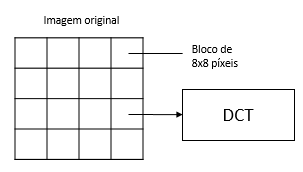
\includegraphics[width=0.9\textwidth]{imagens/dct.png}
        \caption{Codificação baseada na DCT}
    \end{minipage}\hfill
    \begin{minipage}{0.45\textwidth}
        \centering
        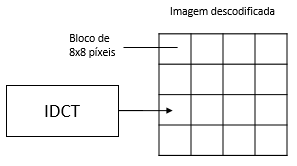
\includegraphics[width=0.9\textwidth]{imagens/idct.png}
        \caption{Descodificação baseada na IDCT}
    \end{minipage}
\end{figure}

Aplicando a codificação representada na Figura 1 à imagem original obtemos os seguintes resultados:

\begin{figure}[h]
	\centering
    \begin{minipage}{0.45\textwidth}
        \centering
        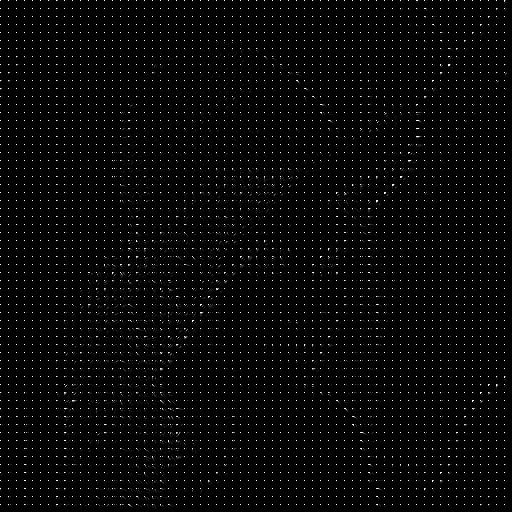
\includegraphics[width=0.7\textwidth]{imagens/dct.jpg}
        \caption{Imagem codificada utilizando a DCT}
    \end{minipage}\hfill
    \begin{minipage}{0.45\textwidth}
        \centering
        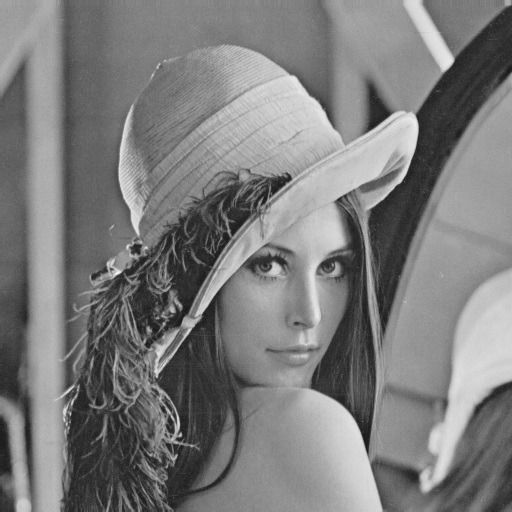
\includegraphics[width=0.7\textwidth]{imagens/idct.jpg}
        \caption{Imagem descodificada utilizando a IDCT}
    \end{minipage}
\end{figure}

Na Figura 3 aplicou-se a DCT $8\times 8$ sobre a imagem, obtendo-se a imagem transformada pela DCT. É de notar que neste ponto ainda não se obteve qualquer compressão. Deve-se notar também que, cada bloco da imagem da Figura 3 possui as maiores amplitudes concentradas em torno do elemento [0,0](canto superior esquerdo). O valor [0,0] designa-se por coeficiente DC, os restantes componentes de um bloco $8\times 8$ são designados de coeficientes AC. É possível observar mais pormenorizadamente estes blocos na Figura 5, onde estão representados 4 blocos $8\times 8$.

\begin{figure}[h]
	\centering
    \begin{minipage}{0.45\textwidth}
        \centering
        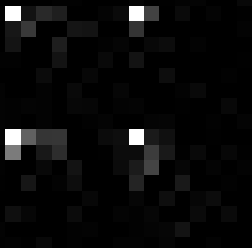
\includegraphics[width=0.7\textwidth]{imagens/blocos.png}
        \caption{Blocos $8\times 8$}
    \end{minipage}\hfill
\end{figure}

\subsection{Codificação/descodificação baseada na DCT com quantificação}
O segundo ponto do trabalho gira em volta da quantificação, o processo de quantificação constitui a forma principal de compressão em qualquer método de compressão com perdas, uma vez que é durante a quantificação que ocorre a \textbf{perda}, ou seja, a eliminação das partes da informação irrelevantes.\\

De uma forma geral, para um bloco com pouca atividade, a maioria dos dados de alta frequência existirá nos coeficientes de ordem inferior, tal como se pode observar na Figura 5. Como se explicou anteriormente, é precisamente o processo de quantificação que conduz à compressão no âmbito de um sistema de codificação baseado na DCT. O processo de quantificação pode exprimir-se pela seguinte expressão:
\begin{center}
$z_{kl} = round(\dfrac{y_{kl}}{q_{kl}})$
\end{center}
onde,\\
\indent \indent $k,l = 0,1,...,7;$\\
\indent \indent $q_{kl}$ representa os elementos da matriz de quantificação Q;\\
\newpage
Na segunda fase do trabalho foi implementada a quantificação, que como referido anteriormente, vai produzir a compressão na imagem. Deste modo foram desenvolvidos dois métodos de codificação e descodificação que realizam as ações descritas no diagrama de blocos da Figura 6.

\begin{figure}[h]
\centering
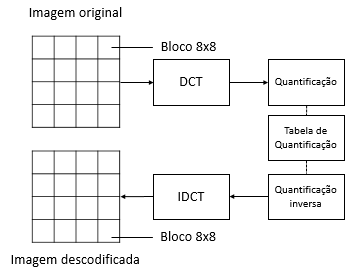
\includegraphics[width=.6\linewidth]{imagens/quant3.png}
\caption{Codificação e descodificação baseada na DCT com quantificação}
\end{figure}

A matriz de quantificação Q $8\times 8$ foi disponibilizada juntamente com o enunciado do trabalho e pode ser observada na Figura 7.

\begin{figure}[h]
	\centering
	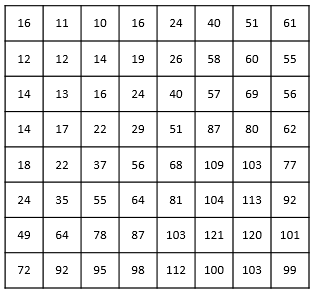
\includegraphics[width=.4\linewidth]{imagens/quantificacao.png}
	\caption{Matriz de quantificação}
\end{figure}

\newpage

\subsubsection{Resultados obtidos}
Implementados os métodos que realizam a codificação e a descodificação, utilizando quantificação, foram obtidos os seguintes resultados, para um fator de qualidade de 75\%.

\begin{figure}[h]
	\centering
    \begin{minipage}{0.45\textwidth}
        \centering
        
\includegraphics[width=0.9\textwidth]{imagens/dct75.jpg}
        \caption{Codificação utilizando DCT com quantificação}
    \end{minipage}\hfill
    \begin{minipage}{0.45\textwidth}
        \centering
        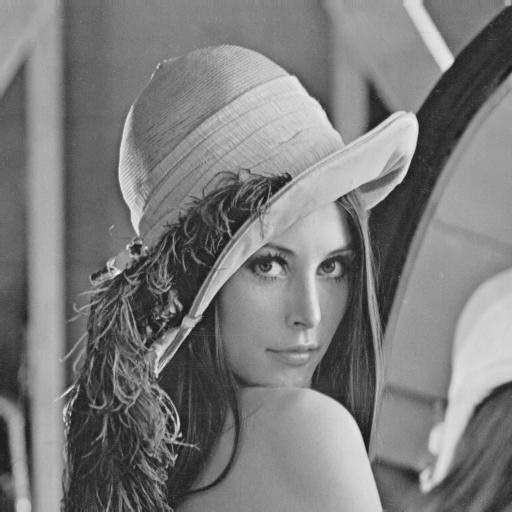
\includegraphics[width=0.9\textwidth]{imagens/idct75.jpg}
        \caption{Descodificação utilizando IDCT com quantificação}
    \end{minipage}
\end{figure}

Comparando os resultados obtidos na Figura 3 e na Figura 8, é possível observar a olho "nu" que os níveis de frequências na Figura 8 são muito menores que na Figura 3. Isto acontece pois a informação irrelevante da imagem é descartada, logo, existe perdas. É possível observar também pela Figura 8, que utilizando um fator de compressão de 75\% conseguimos obter uma imagem descodificada com uma qualidade muito aproximada da imagem original.

Com o diagrama de blocos da Figura 6 implementado, foram efetuados os cálculos  das SNR's (Signal-to-noise ratio) para diferentes fatores de qualidade, respetivamente, 25\%, 50\% e 75\%. A expressão analítica da SNR que foi utilizada define-se do seguinte modo:
\begin{center}
SNR = $10\: log_{10}\: \frac{Psinal}{Pruido}$
\end{center}
A interpretação dos valores da SNR deve fazer-se do seguinte modo:

\begin{itemize}
\item Valores elevados de SNR significam maior qualidade da imagem, isto é, menos distorção.
\item Valores baixos de SNR implicam menor qualidade de imagem, isto é, maior nível de distorção ou perda.
\end{itemize}

Tendo estes dois pontos em consideração podemos observar na Tabela 1 os resultados obtidos de valores de SNR para os diferentes fatores de compressão:

\begin{table}[h]
\centering
\label{my-label}
\begin{tabular}{|c|c|}
\hline
\textbf{Fator de qualidade} & \textbf{Relação sinal-ruído} \\ \hline
25\%                         & 28.06                          \\ \hline
50\%                         & 30.17                          \\ \hline
75\%                         & 32.24                          \\ \hline
\end{tabular}
\caption{Valores de SNR utilizando codificação DCT com quantificação}
\end{table}

Como é possível observar através dos valores obtidos, a relação sinal-ruído é proporcional ao fator de qualidade utilizado, sendo que, quanto maior a qualidade da imagem maior o seu valor de SNR. Um aspeto a ter em conta na norma JPEG deve-se ao facto de, apenas existir perdas na quantificação, logo, na terceira fase do trabalho prático o valores da relação sinal-ruído devem-se manter iguais. Caso isto não aconteça, pode significar problemas na implementação do algoritmo, visto que, a codificação de entropia não introduz perdas na codificação de imagens.

\subsection{Codificação/descodificação com perdas JPEG baseada na DCT}
É possível observar na Figura 10 um diagrama de blocos do codificador JPEG baseado na DCT para uma imagem em tons de cinzento (apenas um componente de cor).

\begin{figure}[h]
\centering
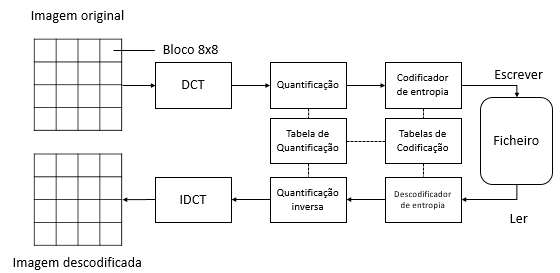
\includegraphics[width=.9\linewidth]{imagens/coddesc.png}
\caption{Diagrama de blocos do codificador/descodificador JPEG}
\end{figure}

Grande parte do processo presente no diagrama de blocos da Figura 9 já foi descrito nos subcapítulos 2.2 e 2.3, logo, a terceira fase do trabalho requer a implementação do codificador de entropia para os valores resultantes da quantificação da imagem.\\
Resumidamente, é realizada a divisão da imagem em blocos de dimensão $8\times 8$ que não se sobrepõem. Em seguida, transforma-se cada bloco de píxeis para o domínio das frequências através de uma transformada DCT (2-D). Os coeficientes que resultam da DCT são posteriormente quantificados e, a seguir, codificados sem perdas por um codificador de entropia.\\
Na norma JPEG, a \textbf{codificação de entropia} consiste em \textbf{duas fases}:

\begin{enumerate}
\item A \textbf{primeira} fase envolve a realização de uma codificação preditiva para o coeficiente DC da DCT quantificada, isto é, para o valor [0,0] da matriz, seguida por uma codificação RL em zig-zag dos coeficientes AC da DCT quantificados.
\item A \textbf{segunda} fase corresponde a uma codificação de entropia dos valores resultantes da primeira fase, que pode ser realizada recorrendo ao método de Huffman.
\end{enumerate}

No que diz respeito ao processo de descodificação de um fluxo de dados JPEG comprimido, o processo é referido na segunda parte no diagrama de blocos da Figura 10. No caso do trabalho prático implementado é realizada uma leitura de um ficheiro de texto onde a imagem foi codificada, seguidamente, os dados referentes ao píxeis da imagem passam por um descodificador de entropia, obtendo-se os coeficientes da DCT quantificados. Com estes valores obtidos é realizada a quantificação inversa explicada anteriormente no subcapítulo 2.3 de modo a obter a imagem descodificada. 

\subsubsection{Codificação de Huffman dos coeficientes DC}
Como referido anteriormente, os coeficientes DC representam os elementos [0,0] da matriz de quantificação, pois estes são os coeficientes com maior frequência. A codificação destes coeficientes é realizado utilizando o DC$_{i}$ e DC$_{i-1}$, para tal, é realizada uma codificação diferencial (DPCM) para estes coeficientes, calculando o diferença entre DC$_{i}$ e DC$_{i-1}$, ou seja, o componente DC atual e o anterior.\\
Com a diferença entre os coeficientes calculada é realizada a sua codificação, para tal, cada diferença passa a ser descrita por dois parâmetros distintos (grandeza, amplitude), a grandeza representa o número de bits necessários para definir a amplitude, e o parâmetro amplitude representa o valor da diferença calculada.\\
Existem duas noções a ter em consideração quando é realizado o calculo da diferença:

\begin{itemize}
 \item Se a diferença for um valor positivo, a amplitude corresponde a esse valor em binário, sendo que, o tamanho desse valor binário será representado pela grandeza.
 \item Se a diferença for um valor negativo, é transformado esse valor para binário e de seguida efetuado o seu complemento, ou seja, os bits que contiverem valor 1 passam a 0 e os que tiverem valor 0 passam a 1, de seguida, é representada a grandeza do mesmo modo descrito anteriormente.
 \end{itemize} 
 
Podemos utilizar como exemplo o primeiro valor de grandeza que obtemos no nosso trabalho, visto que para o primeiro bloco $8\times 8$ da imagem não existe um bloco anterior, então é feita a subtração do coeficiente DC atual por 0. Para um fator de compressão de 75\% o valor do primeiro coeficiente DC é 160, passando o valor 160 para binário é obtida a amplitude 10100000, de seguida, é obtido o comprimento da amplitude que toma o valor 8. Assim, o valor 160 passa a ser descrito pelos parâmetros (8,10100000). O próximo passo é consultar a tabela de Huffman e obter o código para uma grandeza de 8, com este valor obtido o número 160 passa a ser codificado com os bits 11111010100000, grandeza + amplitude. \\
A descodificação dos componentes DC resulta no processo inverso à codificação, ou seja, é descodificado em primeiro lugar a grandeza, desde modo, conseguimos obter o comprimento dos bits que representam a amplitude.

\subsubsection{Codificação de Huffman dos coeficientes AC}
No que diz respeito aos coeficientes AC existem algumas diferenças na sua codificação, tais como os coeficientes DC, estes também são descritos pelos parâmetros (grandeza, amplitude). A grande diferença entre este tipo de codificação e a anterior, deve-se ao facto do modo em que os coeficientes são processados, sendo estes processados em modo de ziguezague. É possível observar este modo na Figura 11:
\newpage
\begin{figure}[h]
\centering
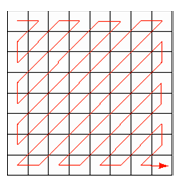
\includegraphics[width=.3\linewidth]{imagens/zigzag.png}
\caption{Processamento em modo ziguezague}
\end{figure}

Os coeficientes AC são processados obtendo o próximo valor de um AC diferente de 0, é então calculada uma \textit{run} que representa o número de coeficientes AC iguais a 0 que precedem o coeficiente não-nulo atual. Deste modo, cada coeficiente passa a ser descrito por os parâmetros (run/grandeza, amplitude). Com estes dois parâmetros obtidos o método de codificação é igual ao dos coeficientes DC. \\

Existem porem algumas particularidades a ter em conta, das quais, as seguintes:

\begin{itemize}
\item Caso o valor de uma \textit{run} seja superior a 15, é utilizado o valor (15/0) de modo a representar uma \textit{run} de 15 zeros, seguido por um zero.
\item É utilizado uma marca EOB (end-of-block) caso todos os coeficientes restantes após um coeficiente não nulo forem nulos, para tal, é utilizado o símbolo 0/0 que é representado pelo valor 1010.
\end{itemize}
\newpage
\subsubsection{Resultados obtidos}
Implementados os métodos que realizam a codificação e a descodificação seguindo o diagrama de blocos da Figura 10, resta apresentar os resultados obtidos e alguns exemplos do funcionamento do algoritmo.\\
Tendo como exemplo o primeiro bloco $8\times 8$ resultante da DCT quantificada da Figura 8, podemos observar a vermelho os coeficientes DC e a verde os coeficiente AC.

\begin{figure}[h]
\centering
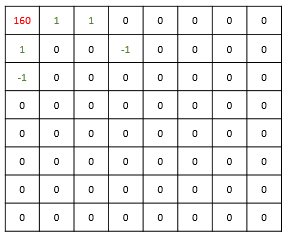
\includegraphics[width=.5\linewidth]{imagens/bloco.png}
\caption{Primeiro bloco $8\times 8$ resultante da DCT}
\end{figure}

Procedendo à codificação deste bloco são obtidos os seguintes resultados:

\begin{itemize}
\item DC: (grandeza, amplitude) [160] = (8, 10100000)
\item AC: [(run/grandeza, amplitude)] = [(0,1),(0,1),(0,-1),(1,1), (7,-1), EOB]
\end{itemize}

Neste caso o resultado final da codificação do primeiro bloco é representado do seguinte modo, onde é possível observar o coeficiente DC codificado, seguido dos 5 coeficientes AC e o bloco de terminação EOB:\\
\begin{center}
111111011010100000 00 001 000 11001 111110100 1010
\end{center}
\newpage
Nas figuras seguintes podemos observar as imagens obtidas dos componentes DCT e das imagens descodificadas, para fatores de qualidade de 25\%, 50\% e 75\%, respetivamente:

\begin{figure}[h]
	\centering
    \begin{minipage}{0.50\textwidth}
        \centering
        
\includegraphics[width=0.5\textwidth]{imagens/ex7/DCT25.png}
    \end{minipage}\hfill
    \begin{minipage}{0.50\textwidth}
        \centering
        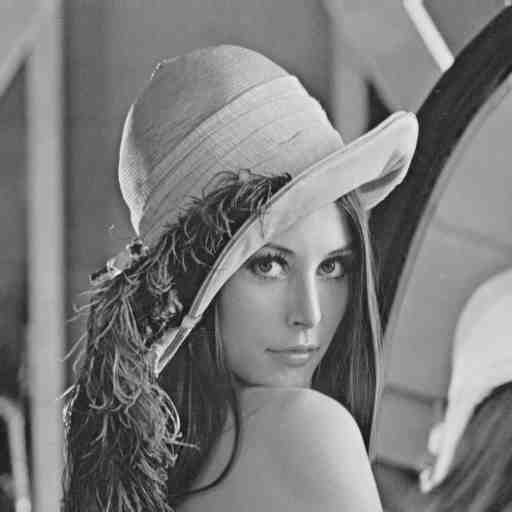
\includegraphics[width=0.5\textwidth]{imagens/ex7/IDCT25.png}
    \end{minipage}
    \caption{DCT e descodificação para um fator de qualidade de 25\%}
\end{figure}
\begin{figure}[h]
	\centering
    \begin{minipage}{0.50\textwidth}
        \centering
        
\includegraphics[width=0.5\textwidth]{imagens/ex7/DCT50.png}
    \end{minipage}\hfill
    \begin{minipage}{0.50\textwidth}
        \centering
        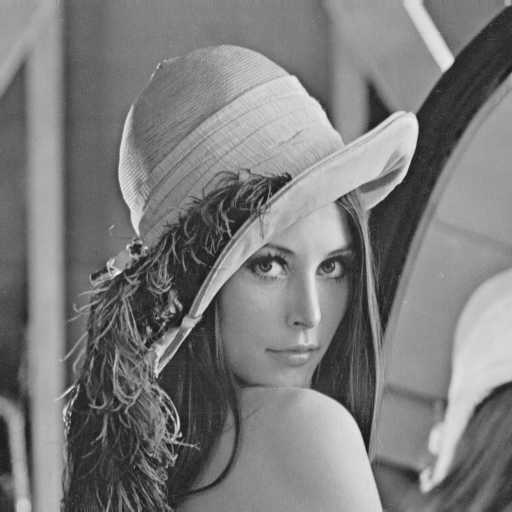
\includegraphics[width=0.5\textwidth]{imagens/ex7/IDCT50.png}
    \end{minipage}
    \caption{DCT e descodificação para um fator de qualidade de 50\%}
\end{figure}
\begin{figure}[h]
	\centering
    \begin{minipage}{0.50\textwidth}
        \centering
        
\includegraphics[width=0.5\textwidth]{imagens/ex7/DCT75.png}
    \end{minipage}\hfill
    \begin{minipage}{0.50\textwidth}
        \centering
        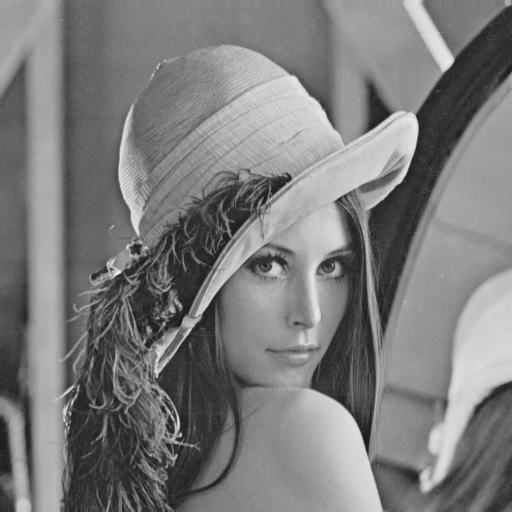
\includegraphics[width=0.5\textwidth]{imagens/ex7/IDCT75.png}
    \end{minipage}
    \caption{DCT e descodificação para um fator de qualidade de 75\%}
\end{figure}

Como é possível observar nas imagens, mesmo com uma fator de qualidade de 25\% a imagem descodificada apresenta uma boa qualidade. De seguida, foram realizado os cálculos das Taxas de Compressão e das SNR's para os diferentes valores de compressão, sendo possível observar os valores na Tabela 2:
\newpage
\begin{table}[]
\centering
\begin{tabular}{|c|c|c|c|}
\hline
\textbf{Fator de Compressão}     & \textbf{25\%} & \textbf{50\%} & \textbf{75\%} \\ \hline
\textbf{Relação Sinal-Ruído}     & 28.06         & 30.17         & 32.24         \\ \hline
\textbf{Taxa de Compressão}      & 5.34          & 4.61          & 4.26          \\ \hline
\textbf{Tempo de Codificação}    & 1.53          & 2.16          & 3.06          \\ \hline
\textbf{Tempo de Descodificação} & 1.63          & 2.06          & 2.91          \\ \hline
\end{tabular}
\caption{Resultados obtidos}
\label{my-label}
\end{table}

Observado os resultados obtidos na Tabela 2 podemos retirar as seguintes conclusões:
\begin{itemize}
\item No que diz respeito aos valores obtidos na SNR podemos confirmar que são idênticos aos valores do capitulo 2.3, logo, não existiu perda de informação na codificação de entropia, apenas na quantificação. Ou seja, os resultados são os esperados.
\item No que diz respeito à Taxa de Compressão seria de esperar que à medida que o fator de qualidade aumentasse a Taxa de Compressão diminuiria, visto que, quanto mais aproximada a imagem descodificada for da imagem original, mais o valor da Taxa de Compressão se aproxima de 1.
\item Por fim, os Tempos de Codificação/Descodificação são relativamente baixos, salientando o facto de existir um aumento proporcional ao fator de qualidade, isto devesse ao facto de existirem mais amostrar para quantificar.
\end{itemize}

É possível ainda reforçar o que foi referido nos pontos anteriores com o gráfico presente na Figura 15, que representa a Taxa de Compressão em função da SNR.
\newpage
\begin{figure}[h]
	\centering
    \begin{minipage}{0.50\textwidth}
        \centering
        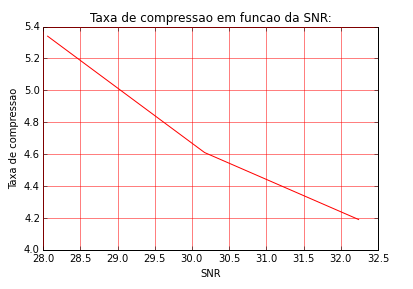
\includegraphics[width=1.2\textwidth]{imagens/graph.png}
    \end{minipage}\hfill
    \caption{Taxa de Compressão em função da SNR}
\end{figure}
\newpage
\section{Conclusões}
Com a finalização do trabalho e os resultados obtidos analisados podemos concluir que o trabalho foi implementado com sucesso. Os valores referentes às SNR's e Taxas de Compressão são os pretendidos e mesmo com um fator de compressão de 25\% é possível obter uma qualidade de imagem muito aproximada da original, apenas quando se desce o fator de qualidade para os 10/15\% é que se deixa de ter uma qualidade aceitável. No que diz respeito aos tempos de processamento estes mantiveram-se relativamente baixos, como referido anteriormente, sendo que podem existir otimizações no desenvolvimento do código de modo a reduzir ainda mais estes tempos. Em suma o grupo obteve conhecimentos referentes à compressão de imagens digitais e o funcionamento da norma JPEG. 
\end{document}